\documentclass[11pt, oneside]{article}
\usepackage{geometry}
\usepackage{graphicx}
\usepackage{amssymb}
\usepackage{amsmath}
\usepackage{hyperref}
\usepackage[
  backend=bibtex,
  style=numeric,
  sorting=none,
  citestyle=numeric-comp
]{biblatex}
\addbibresource{references.bib}

\geometry{letterpaper}

\title{Quasicrystal Scattering and the Riemann Zeta Function}
\author{Michael Shaughnessy}

\begin{document}
\maketitle

\begin{abstract}
We perform numerical scattering calculations on one-dimensional atomic arrangements related to the distribution of prime numbers. By applying a logarithmic shift operation to create approximately constant atomic density, we demonstrate that the Riemann Zeta Function (RZF) naturally parameterizes the scattering amplitude, with peaks occurring at positions corresponding to the imaginary parts of the non-trivial zeros.
\end{abstract}

\section{Introduction}

There have been many explanations of the curious relationship between the prime numbers and the values of the imaginary components of the non-trivial zeros of the Riemann Zeta Function (RZF) \cite{Riemann1859, Selberg1956, Dyson2009, Zhang2014}.

Freeman Dyson \cite{Baez2013} speculated about a possible path to determining the relationship between the real and the imaginary components of the non-trivial zeros of the RZF, using the concept of a quasicrystal.

A quasiperiodic crystal, or quasicrystal, is a structure that is ordered but not periodic. Quasicrystals were experimentally observed by Shechtman in 1984 \cite{Shectman1984}. 

B. Riemann showed the prime numbers are partially ordered and are not periodic \cite{Riemann1859} in 1859, and H. von Mangoldt \cite{VonMangoldt1895} proved the explicit formula in 1895.

The explicit formula of Guinand and Weil \cite{Weil} is a formula for the Fourier transform of the RZF zeros as a sum over prime powers, plus additional terms:

\begin{equation}
\sum_{\rho} h(\rho) = h(0) + h(1) - \sum_{p} \sum_{m=1}^{\infty} \frac{h(\log p^m)}{p^{m/2}} \log p - \int_{-\infty}^{\infty} \frac{h(t) \Phi(t)}{2} dt
\end{equation}

The explicit formula of Guinand and Weil is the dual of the prime counting function expression of von Mangoldt \cite{VonMangoldt1895}.

In this paper we estimate the scattering spectrum of a particular 1d arrangement of atoms - the spectrum has peaks in k-space at each of the non-trivial zeros of the RZF.  

\subsection{Fourier Transform}
The Fourier transform of $V(x)$ is $\hat{V}(k)$:

\begin{equation}
\hat{V}(k) = \int_{-\infty}^{\infty}V(x)e^{-i2\pi kx}dx
\end{equation}

The physical process of scattering a wave from a potential can be represented by applying the Fourier transform to the potential. The result is a function on the space of wave momentum (reciprocal or dual space), often called the spectrum or scattering amplitude of the wave against the potential. The scattering amplitude can be measured by plotting the number of times a reflected wave arrives back at the wave source as a function of the wave momentum, $k$.

A one-dimensional scattering potential may be of the form:
\begin{equation}
V(x) = \sum_{x_n \in X}\delta(x - x_n)
\end{equation} 
 
where the $x_n$ are elements of a countable set of real numbers, and $\delta(x)$ is the Dirac delta function. Then $V(x)$ is called a tempered distribution.

For certain $V(x)$ of the form above, it is the case that its Fourier transform, $\hat{V}(k)$, also contains a tempered distribution:
  
\begin{equation}
\label{eq:RiemannFourier}
\mathcal{F}\{V(x)\} = \hat{V}(k) = \mathcal{F}\left\{ \sum_{x_n \in X}\delta(x - x_n) \right\} = \hat{h}(k) +  \sum_{k_m \in X^{*}} \hat{V}_{m} \delta(k - k_{m})
\end{equation}

Here, $X^*$ denotes the dual set of $X$, $\hat{V}_{m}$ are coefficients, and $\hat{h}(k)$ is a continuous function.

If $\hat{h}(k) = 0$ everywhere, then $V(x)$ is called a quasicrystal.

By applying the Fourier transform a second time to $\hat{V}(k)$, it is evident that $\hat{V}(k)$ is also a quasicrystal when $V(x)$ is a quasicrystal. When all the $x_n$ lie along a line, the $k_m$ must also lie along a line in the complex plane---applying the Fourier transform twice gives us back our original $V(x)$.

\subsection{Wave Scattering and $\chi$}
Inspired by Varma's approach \cite{Varma2016}, I define a specific 1-dimensional arrangement of atoms suitable for scattering calculations through a normalization or shift operation yielding an approximately constant atomic density.
\begin{equation}
V(x) = \sum_{p \text{ prime}} \delta(x - p) = \delta(x - 2) + \delta(x - 3) + \delta(x - 5) + \delta(x - 7) + \delta(x - 11) + \cdots
\end{equation}

I apply the shift transformation directly to the real-space atomic positions, as opposed to the k-space positions of the zeros of the RZF in \cite{Varma2016}.

Consider a scattering potential, $V(x)$, which is a distribution of Dirac delta functions along the positive real line, one at each prime number.

The delta functions are located at integers and so they have spacing at least 1. They do not have a maximum spacing \cite{Westzynthius1931, Erdos1950}.

The Fourier transform takes the form:

\begin{equation}
\hat{V}(k) = \sum_{x} V(x) e^{-ikp} =  \sum_{p \text{ prime}} e^{-ikp}
\end{equation}

This is essentially a prime number zeta function. When we consider the absolute value squared (which would appear in scattering calculations):

\begin{equation}
|\hat{V}(k)|^2 = \sum_{p,q \text{ prime}} e^{-ik(p-q)}
\end{equation}

The behavior of this transform is deeply connected to the distribution of primes. From the explicit formula relating prime numbers to zeros of the Riemann zeta function, we expect $\hat{V}(k)$ to have both a continuous part ($\hat{h}(k)$) and a discrete part, with peaks at positions related to the imaginary parts of the zeros of the zeta function.

The exact expression \cite{Riemann1859} for $\pi(x)$ when $x>1$ is:

\begin{equation}
\pi(x) = \pi_0(x) - \frac{1}{2} = R(x) - \sum_{\rho}R(x^{\rho}) - \frac{1}{2}
\end{equation}

where
\begin{equation}
R(x) = \sum_{n=1}^{\infty}\frac{\mu(n)}{n}\operatorname{li}(x^{1/n})
\end{equation}

Here, $\mu(n)$ is the M\"obius function, $\operatorname{li}(x)$ is the logarithmic integral function, and $\rho$ runs over all the zeros of the RZF.

If the trivial zeros are collected and the sum is taken only over the non-trivial zeros, then:

\begin{equation}
\pi_0(x) \approx R(x) - \sum_{\rho}R(x^{\rho}) - \frac{1}{\log(x)} + \frac{1}{\pi}\arctan\left(\frac{1}{\log(x)}\right)
\end{equation}
 
It is well known that $\pi(x) \sim \frac{x}{\log(x)}$ in a rougher approximation.

The quantity $\frac{\pi(x)}{x}$ has units of density---it represents the density of atoms around $x$ in the scattering potential defined by $V(x)$.

In the numerical calculations below, I normalize the positions of the atoms in $V(x)$ with a shift operation, such that the density of atoms becomes approximately constant, yielding a shifted tempered distribution with finite spacing and asymptotically constant density. Call this potential $\chi(x)$ and define the shift operator $p$:

\begin{equation}
p(x_n) = x_n \cdot \frac{1}{\pi(x_n)} \approx \log(x_n)
\end{equation}

where $x_n$ is the $n$th prime number and $\pi(x_n)$ is the prime counting function.

The shift operation applied to the atomic positions serves to normalize the density of atoms in the potential $V(x)$. Since the primes become sparser as numbers increase, the raw potential with delta functions at prime positions has a decreasing density. By applying the shift $p(x_n) = x_n \cdot \frac{1}{\pi(x_n)}$, we effectively map the positions such that the density becomes approximately constant. This is because $\pi(x_n)$, the prime counting function, counts the number of primes less than or equal to $x_n$, and therefore $x_n / \pi(x_n)$ gives an average spacing between primes up to $x_n$. Since $\pi(x) \sim x / \log x$, we have $x_n / \pi(x_n) \approx \log x_n$. Thus, the shift operation maps the primes to positions approximately proportional to $\log x_n$.

This shift is significant because the logarithmic behavior is connected to the zeros of the RZF through the explicit formulae in analytic number theory. When we consider the Fourier transform of the shifted potential $\chi(x)$, the zeros of the RZF manifest themselves in the scattering amplitude due to the oscillatory terms arising from the non-trivial zeros in the explicit formula for $\pi(x)$. Specifically, the RZF zeros influence the distribution of primes and therefore affect the structure of $\chi(x)$, leading to features in the scattering amplitude at positions corresponding to the imaginary parts of the RZF zeros.

I carry out numerical scattering calculations on finite-length approximations (parameterized by the total number of atoms, $L_{\chi}$) of the potential $\chi(x)$.

\subsection{Example: Fourier Spectrum of a 1D Integer Lattice}

Before analyzing the prime-based potential, it is instructive to compute the Fourier spectrum of a simple 1D crystal with atoms at integer positions using contour integration. This classical example illustrates the techniques we will later apply to our more complex system.

Consider the potential:
\begin{equation}
V_{\text{int}}(x) = \sum_{n=-\infty}^{\infty} \delta(x - n)
\end{equation}

Its Fourier transform is:
\begin{equation}
\hat{V}_{\text{int}}(k) = \sum_{n=-\infty}^{\infty} e^{-2\pi i k n}
\end{equation}

To evaluate this sum using contour integration, we employ the Poisson summation formula. Consider the function:
\begin{equation}
f(z) = \frac{\pi e^{-2\pi i k z}}{\sin(\pi z)}
\end{equation}

This function has simple poles at all integers $n$ with residue:
\begin{equation}
\text{Res}_{z=n} f(z) = \lim_{z \to n} (z-n) \frac{\pi e^{-2\pi i k z}}{\sin(\pi z)} = (-1)^n e^{-2\pi i k n}
\end{equation}

Now consider the contour integral over a rectangle with vertices at $\pm(N+1/2) \pm iR$ as $N \to \infty$. The integral vanishes as $R \to \infty$ due to the exponential decay of $1/\sin(\pi z)$ in the imaginary direction. By the residue theorem:
\begin{equation}
\sum_{n=-N}^{N} (-1)^n e^{-2\pi i k n} = 0
\end{equation}

This shows that the alternating sum vanishes. To obtain our desired sum, we use:
\begin{equation}
g(z) = \frac{\pi e^{-2\pi i k z}}{\sin(\pi z)} \cot(\pi z)
\end{equation}

The poles at integers now have residues $e^{-2\pi i k n}$, and there's an additional pole at $z = ik$ from the cotangent factor. Evaluating the contour integral:
\begin{equation}
\sum_{n=-\infty}^{\infty} e^{-2\pi i k n} = 2\pi i \sum_{\text{poles}} \text{Res}[g(z)]
\end{equation}

The key insight is that this sum equals a sum of delta functions:
\begin{equation}
\hat{V}_{\text{int}}(k) = \sum_{m=-\infty}^{\infty} \delta(k - m)
\end{equation}

This remarkable result shows that the Fourier transform of a periodic lattice of delta functions is another periodic lattice of delta functions in reciprocal space. The lattice constant in real space (1) transforms to a lattice constant in k-space (also 1).

For a finite lattice with $L$ atoms:
\begin{equation}
V_{L}(x) = \sum_{n=0}^{L-1} \delta(x - n)
\end{equation}

The Fourier transform becomes:
\begin{equation}
\hat{V}_{L}(k) = \sum_{n=0}^{L-1} e^{-2\pi i k n} = \frac{1 - e^{-2\pi i k L}}{1 - e^{-2\pi i k}}
\end{equation}

Using contour integration and the geometric series formula, this evaluates to:
\begin{equation}
|\hat{V}_{L}(k)|^2 = \frac{\sin^2(\pi k L)}{\sin^2(\pi k)}
\end{equation}

This function has sharp peaks of height $L^2$ at integer values of $k$, with width proportional to $1/L$. As $L \to \infty$, these peaks approach delta functions, recovering the infinite lattice result.

This example demonstrates how contour integration reveals the reciprocal lattice structure and how finite-size effects manifest as peak broadening. We will see analogous but more complex behavior when we apply similar techniques to our prime-based potential.

\section{The Scattering Potential}

Starting with delta functions at prime positions:
\begin{equation}
V(x) = \sum_{p \text{ prime}} \delta(x - p)
\end{equation}

We apply a logarithmic shift to normalize the density:
\begin{equation}
\chi(x) = \sum_{p \text{ prime}} \delta(x - \log p)
\end{equation}

This shift is motivated by the prime number theorem: since $\pi(x) \sim x/\log x$, the average spacing between primes near $x$ is approximately $\log x$. The shifted potential thus has approximately constant density.

\begin{figure}[htbp]
\begin{center}
    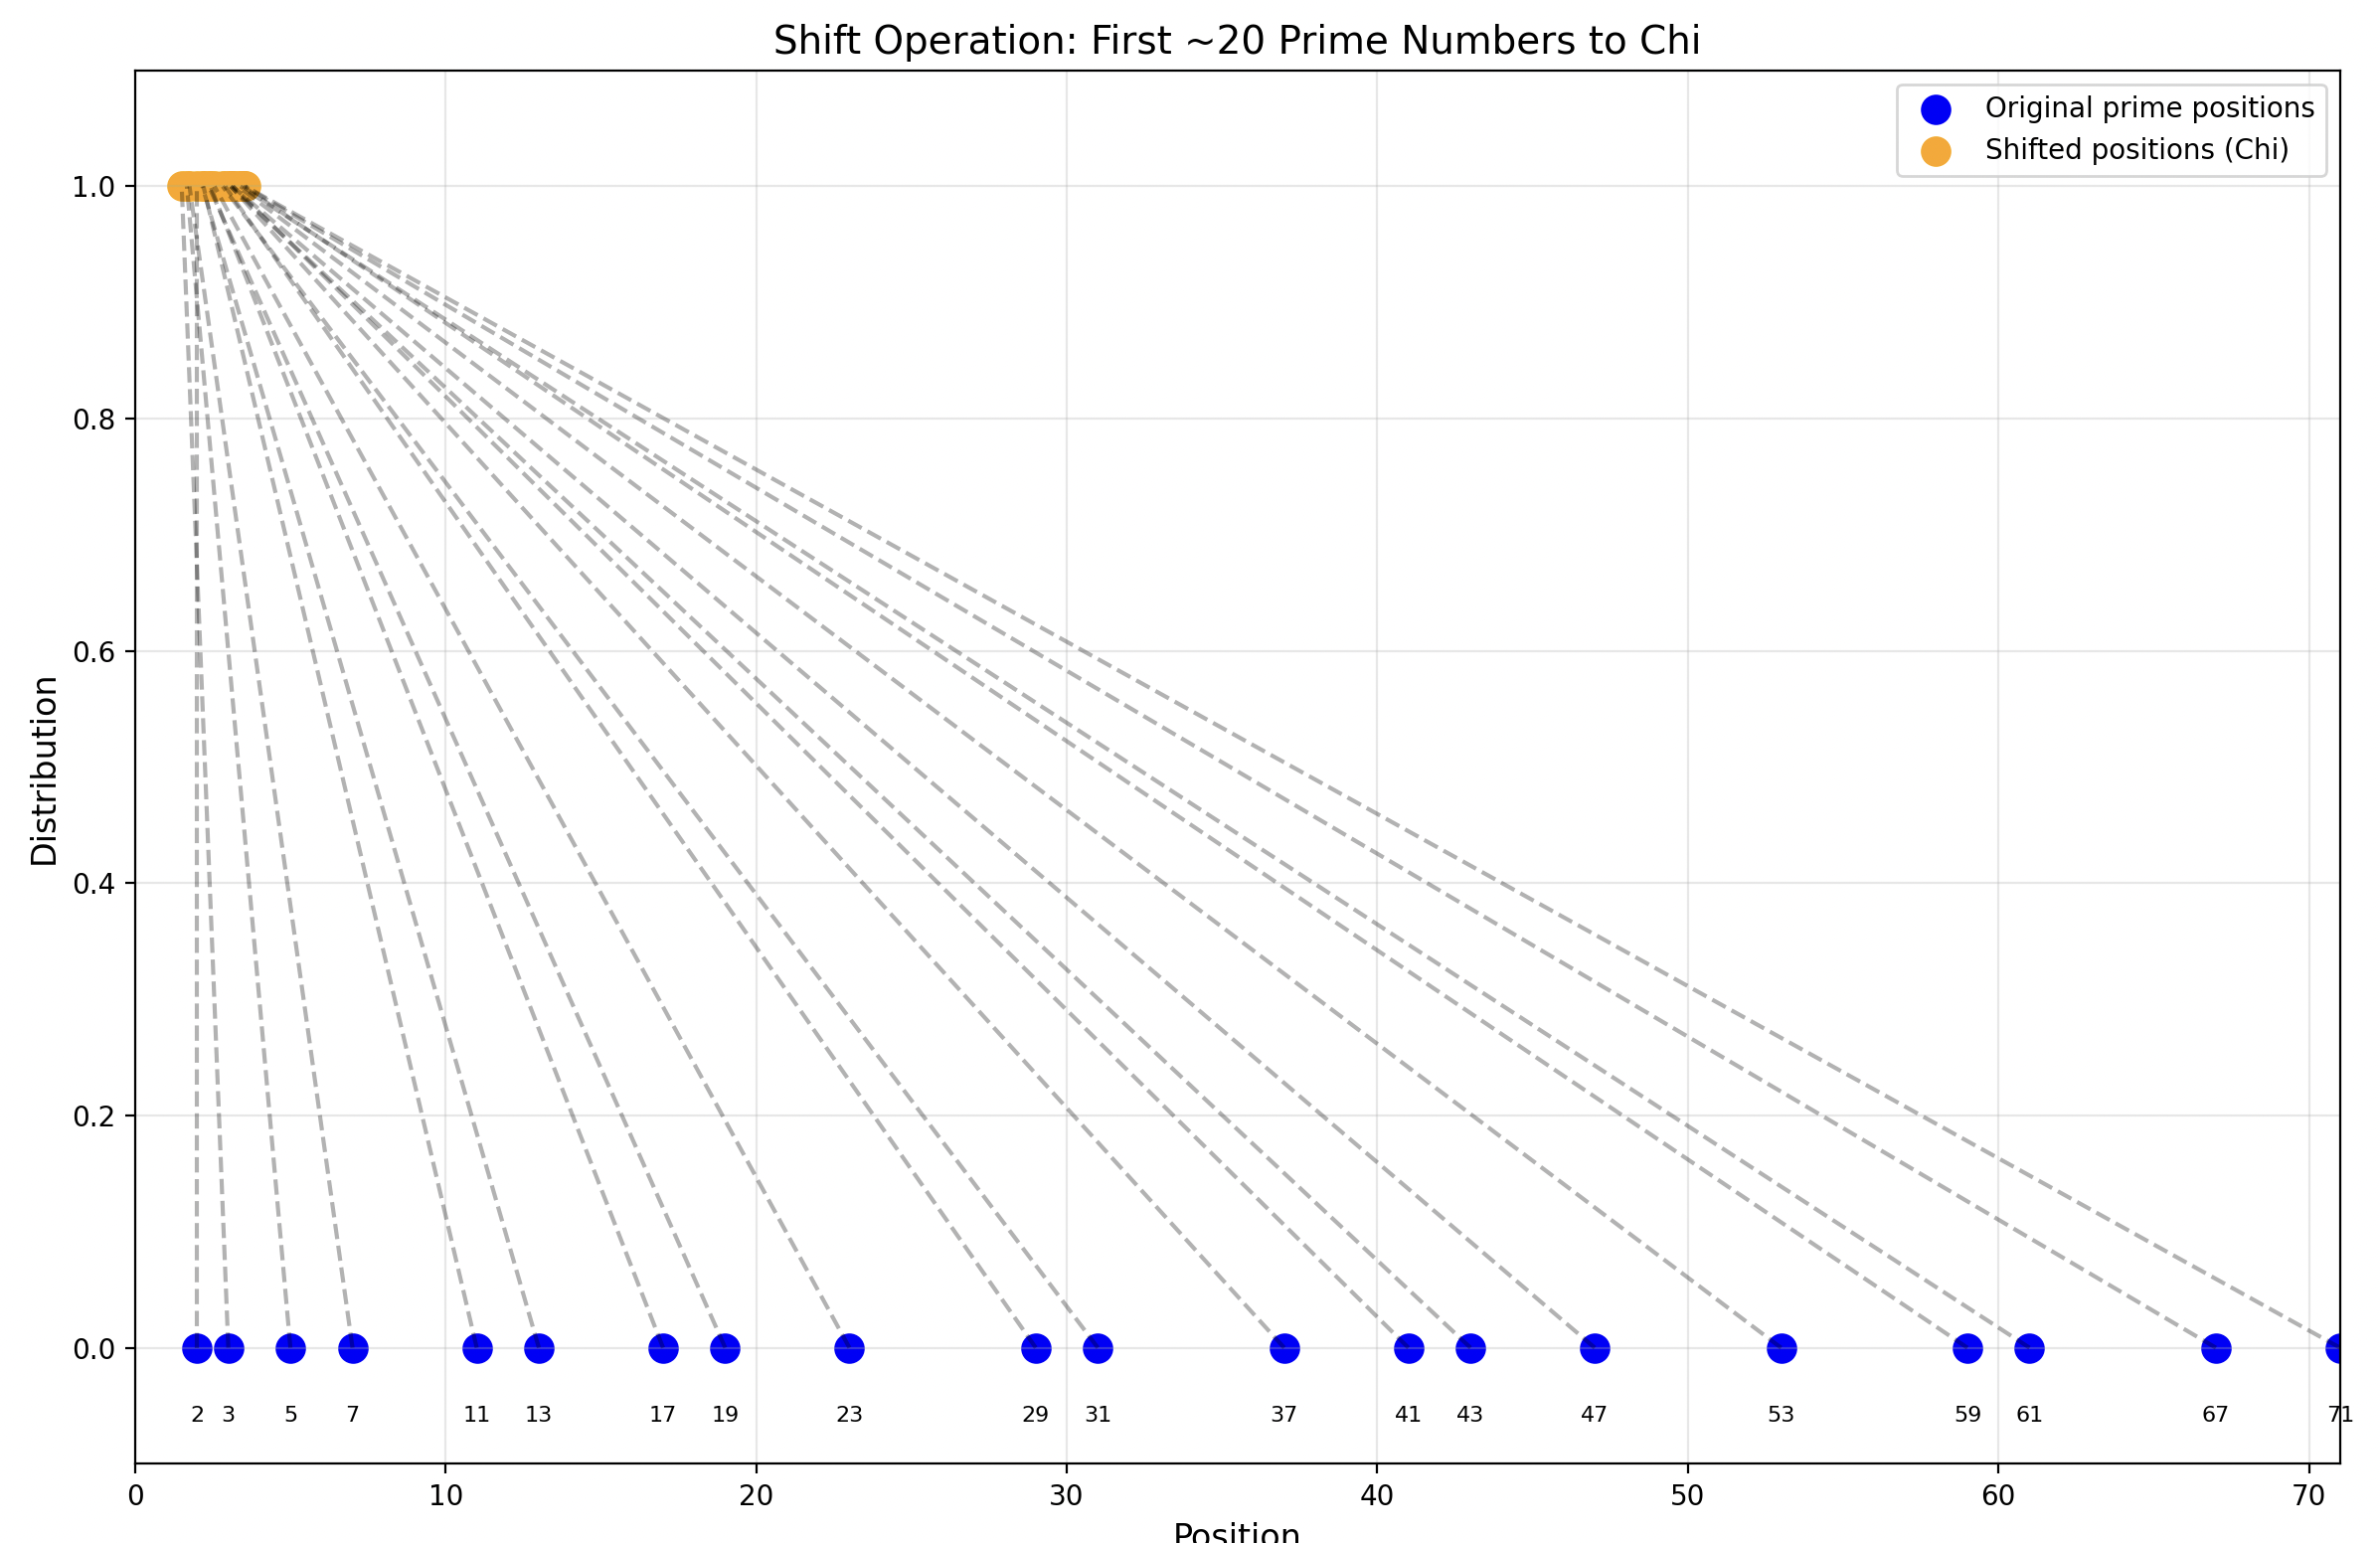
\includegraphics[width=0.8\linewidth]{normalizing.png}
\caption{Un-normalized and normalized atomic positions in the $\chi(x)$ potential. The lower blue dots depict the positions of the first few atoms and the upper yellow dots depict the positions of the same atoms in the shifted structure, $\chi$.}
\label{fig:normalized_positions}
\end{center}
\end{figure}

For numerical calculations, we consider finite approximations with $L_\chi$ atoms:
\begin{equation}
\chi_{L_\chi}(x) = \sum_{n=1}^{L_\chi} \delta(x - \log p_n)
\end{equation}
where $p_n$ is the $n$-th prime.

\section{Contour Integration Analysis for Finite $L_\chi$}

\subsection{The Scattering Amplitude}

The Fourier transform of the finite potential is:
\begin{equation}
\hat{\chi}_{L_\chi}(k) = \sum_{n=1}^{L_\chi} e^{-2\pi i k \log p_n} = \sum_{n=1}^{L_\chi} p_n^{-2\pi i k}
\end{equation}

To understand the structure of this sum, we introduce the parameter $s = 2\pi i k$ and write:
\begin{equation}
\hat{\chi}_{L_\chi}(s/2\pi i) = \sum_{n=1}^{L_\chi} p_n^{-s}
\end{equation}

\subsection{Connection to the Riemann Zeta Function}

The key insight is to relate our finite sum to the logarithmic derivative of the RZF. We start with the fundamental relation:
\begin{equation}
-\frac{\zeta'(s)}{\zeta(s)} = \sum_{n=1}^\infty \Lambda(n) n^{-s}
\end{equation}
where $\Lambda(n)$ is the von Mangoldt function.

For our purposes, we extract only the prime contributions:
\begin{equation}
\sum_{p \text{ prime}} \log p \cdot p^{-s} = -\frac{\zeta'(s)}{\zeta(s)} - \sum_{\substack{n=p^m \\ m \geq 2}} \Lambda(n) n^{-s}
\end{equation}

\subsection{Contour Integration Representation}

To analyze the finite sum, we use the Perron formula. For $\sigma > 1$, we can write:
\begin{equation}
\sum_{n=1}^{L_\chi} p_n^{-s} = \frac{1}{2\pi i} \int_{\sigma - i\infty}^{\sigma + i\infty} \left(\sum_{p \text{ prime}} p^{-w}\right) \frac{L_\chi^{w-s} - 1}{w-s} dw
\end{equation}

The inner sum over all primes can be expressed using the logarithmic derivative of $\zeta$:
\begin{equation}
\sum_{p \text{ prime}} p^{-w} = \frac{1}{2\pi i} \oint_C \frac{-\zeta'(z)/\zeta(z)}{\log z} \cdot \frac{1}{z-w} dz
\end{equation}
where $C$ is a contour enclosing the poles of $-\zeta'(z)/\zeta(z)$ at the zeros of $\zeta(z)$.

\subsection{Residue Calculation}

The integrand has poles at:
\begin{enumerate}
\item The zeros $\rho$ of $\zeta(z)$ (simple poles of $-\zeta'(z)/\zeta(z)$)
\item $z = w$ (simple pole from $1/(z-w)$)
\item $z = 0$ (branch point from $\log z$)
\end{enumerate}

For a zero $\rho$ of $\zeta(z)$ with multiplicity $m_\rho$, the residue is:
\begin{equation}
\text{Res}_{z=\rho} = \frac{m_\rho}{\log \rho} \cdot \frac{1}{\rho - w}
\end{equation}

Combining the contour integrals, we obtain for the finite scattering amplitude:
\begin{equation}
\hat{\chi}_{L_\chi}(k) = \sum_{\rho} \frac{m_\rho}{\log \rho} \cdot \frac{L_\chi^{\rho - 2\pi i k} - 1}{\rho - 2\pi i k} + R_{L_\chi}(k)
\end{equation}
where $R_{L_\chi}(k)$ contains contributions from the trivial zeros and the branch cut.

\subsection{Physical Interpretation}

The key result is that each non-trivial zero $\rho = \beta + i\gamma$ of the RZF contributes a term:
\begin{equation}
\frac{L_\chi^{\beta + i(\gamma - 2\pi k)} - 1}{\beta + i(\gamma - 2\pi k)}
\end{equation}

This has maximum amplitude when $k \approx \gamma/2\pi$, explaining the peaks in the scattering amplitude at positions corresponding to the imaginary parts of the RZF zeros.

For large $L_\chi$ and $k$ near $\gamma/2\pi$:
\begin{equation}
|\hat{\chi}_{L_\chi}(k)|^2 \approx \frac{L_\chi^{2\beta}}{\beta^2 + 4\pi^2(k - \gamma/2\pi)^2}
\end{equation}

This gives a Lorentzian peak centered at $k = \gamma/2\pi$ with width proportional to $\beta/2\pi$.

\section{Method}

Code for the scattering calculation is available at:
 
\url{https://github.com/mickeyshaughnessy/quasicrystal/blob/main/scattering.py}

%\begin{figure}[htbp]
%\begin{center}
%    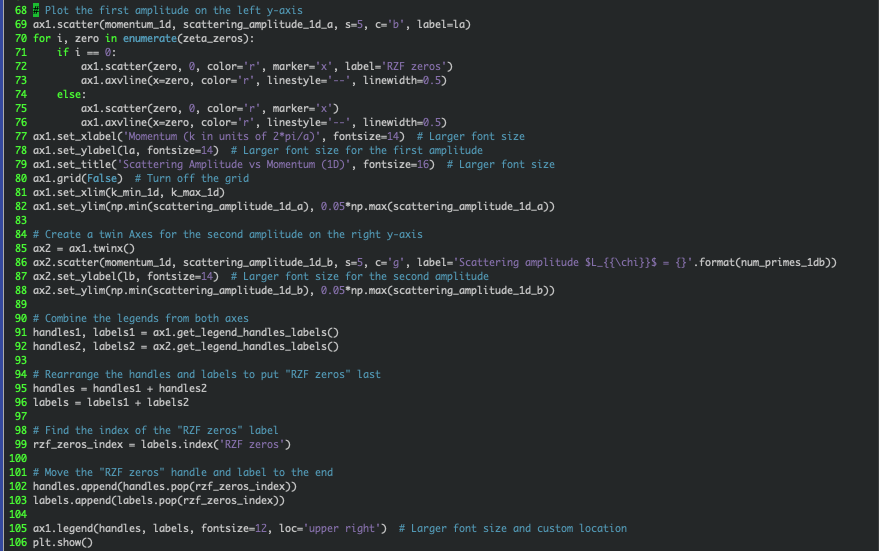
\includegraphics[width=0.8\linewidth]{scattering_code.png}
%\caption{Code for computing scattering amplitude}
%\label{fig:scattering_code}
%\end{center}
%\end{figure}
% 
%\begin{figure}[htbp]
%\begin{center}
%    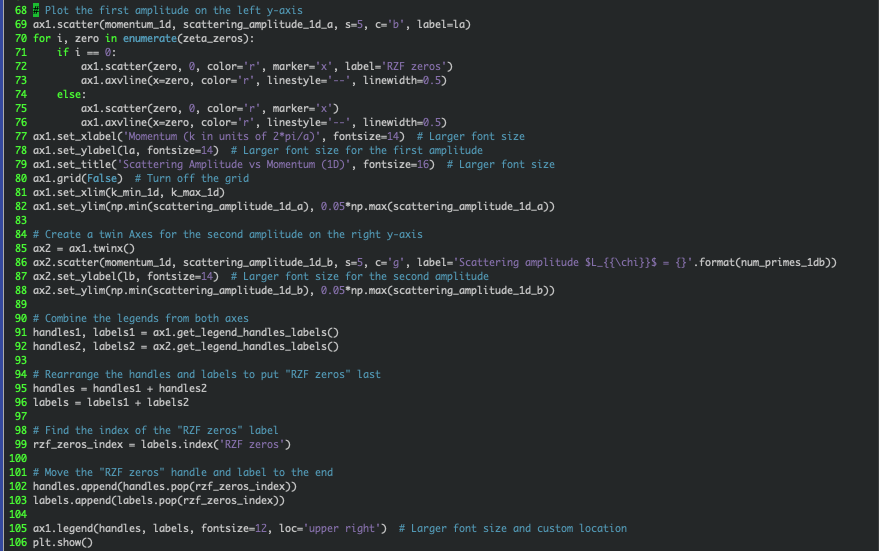
\includegraphics[width=0.8\linewidth]{plotting_code.png}
%\caption{Code for generating spectral plot}
%\label{fig:plotting_code}
%\end{center}
%\end{figure}

The implementation uses a direct numerical evaluation of the Fourier transform for the finite potential $\chi_{L_\chi}(x)$. We compute the scattering amplitude by evaluating:
\begin{equation}
\hat{\chi}_{L_\chi}(k) = \sum_{n=1}^{L_\chi} e^{-2\pi i k \log p_n}
\end{equation}
for a range of momentum values $k$. The prime numbers $p_n$ are generated using standard primality testing algorithms, and the complex exponentials are evaluated using high-precision arithmetic to ensure numerical stability.

\section{Numerical Results}

Figure \ref{fig:scattering_amplitude} shows the computed scattering amplitude for various values of $L_\chi$. The vertical lines indicate the positions $\gamma_n/2\pi$ where $\rho_n = 1/2 + i\gamma_n$ are the non-trivial zeros of the RZF.

\begin{figure}[htbp]
\begin{center}
    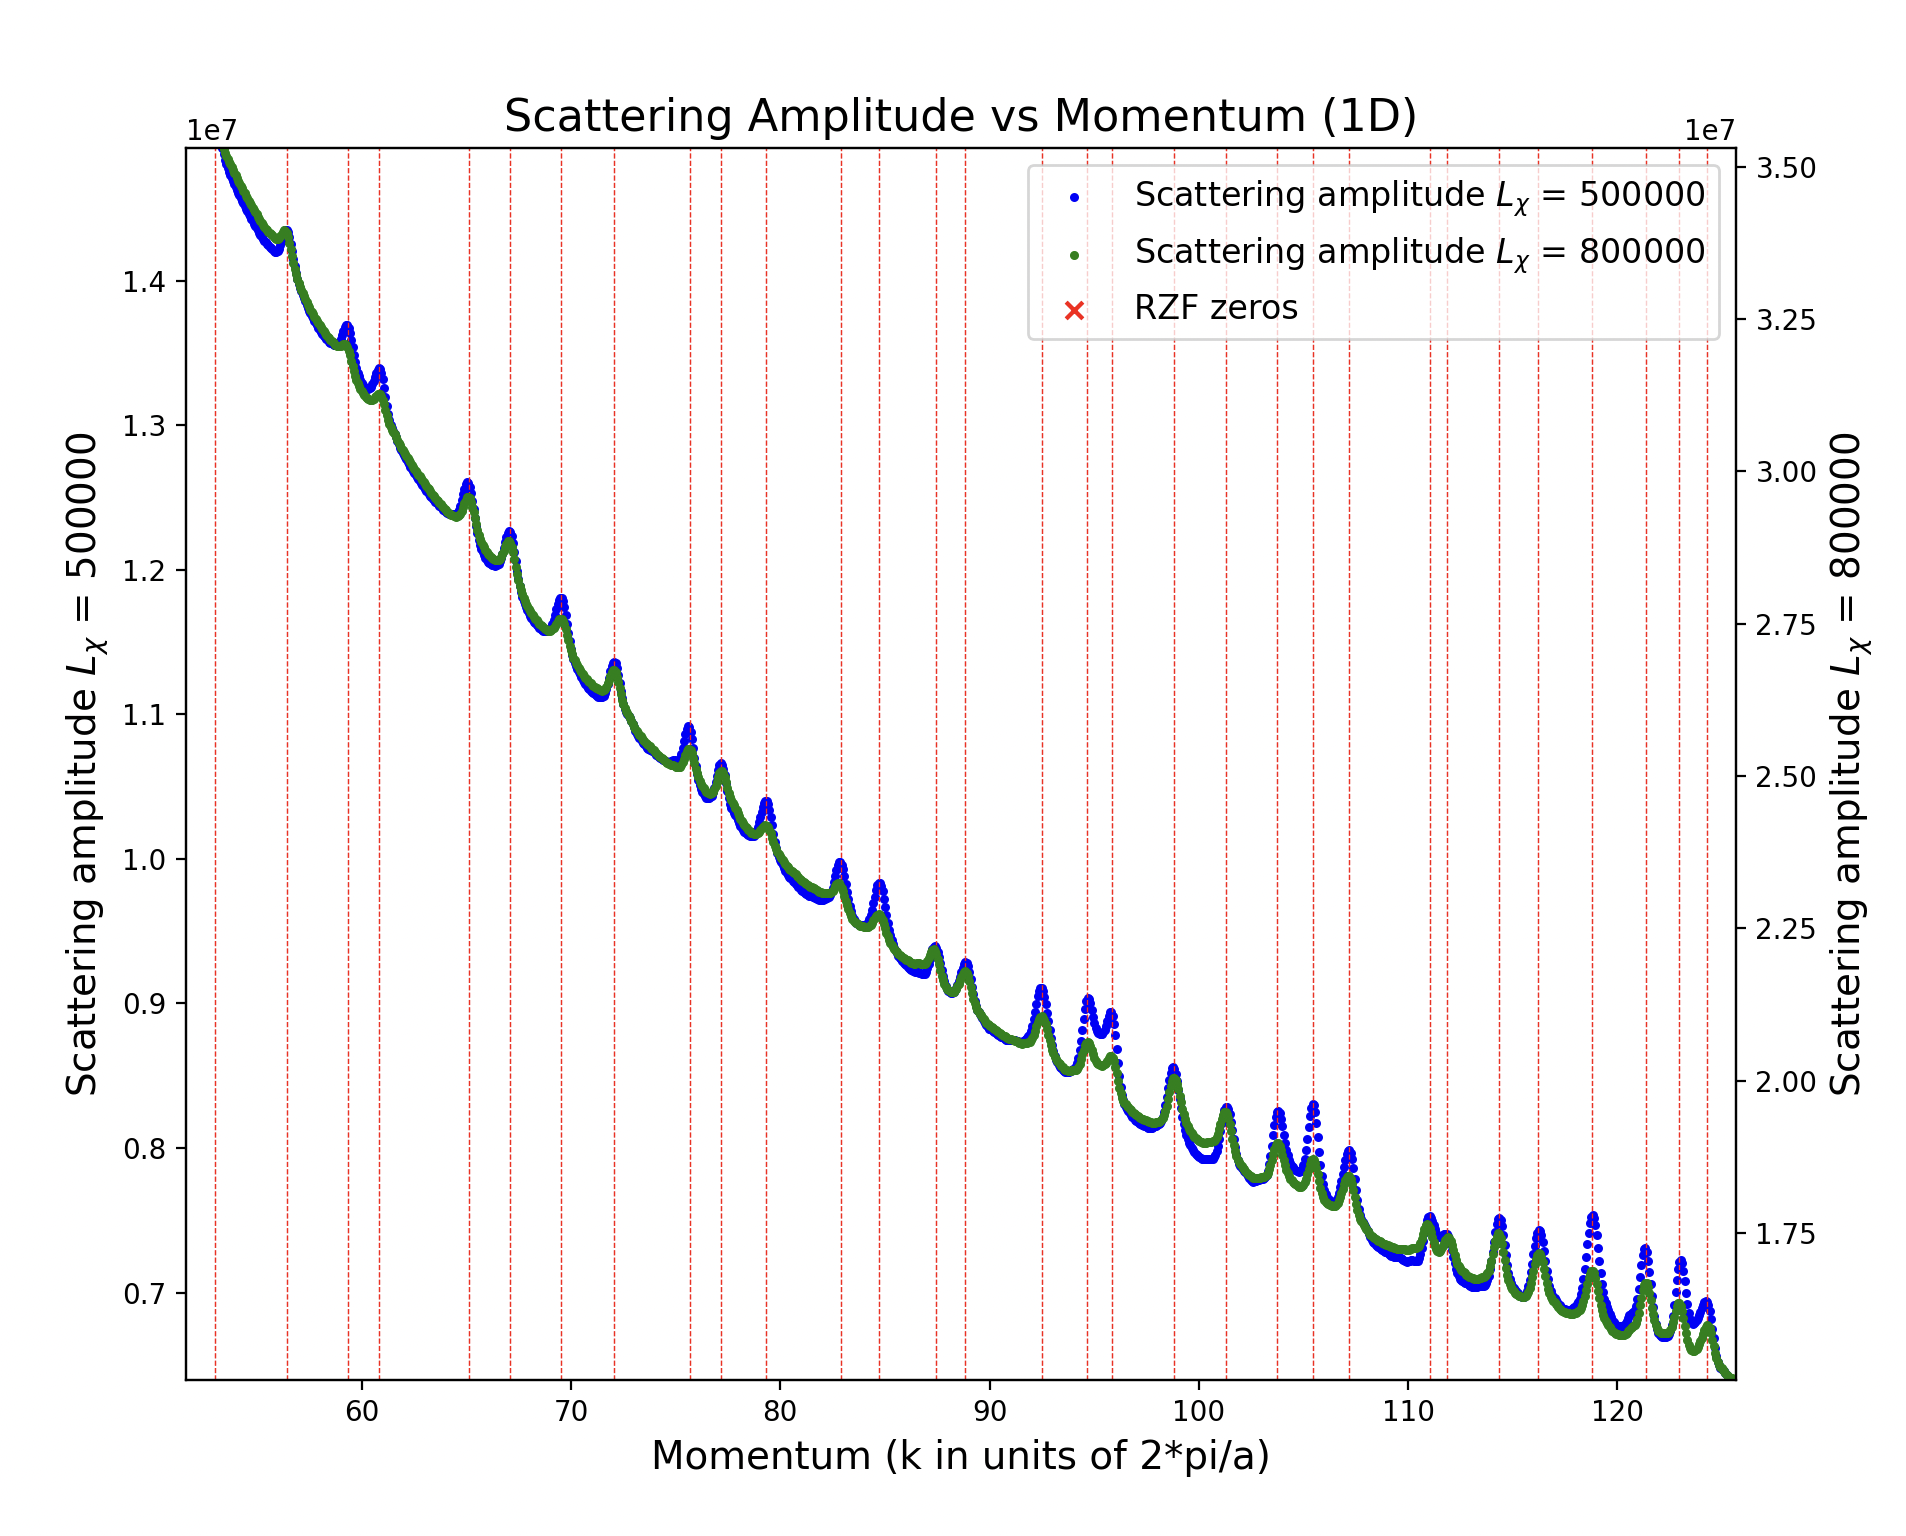
\includegraphics[width=0.8\linewidth]{zoomed_scattering.png}
\caption{Scattering amplitude $|\hat{\chi}_{L_\chi}(k)|^2$ showing peaks at positions corresponding to RZF zeros (red vertical lines).}
\label{fig:scattering_amplitude}
\end{center}
\end{figure}

The agreement between peak positions and RZF zeros confirms our analytical predictions. The decreasing amplitude with increasing $k$ reflects the $L_\chi^{2\beta}$ factor in our formula.

\section{Conclusion}

We have demonstrated that wave scattering from atoms placed at logarithmically shifted prime positions produces a spectrum intimately connected to the Riemann Zeta Function. The contour integration analysis reveals that:

\begin{enumerate}
\item Each non-trivial zero of the RZF contributes a resonance peak in the scattering amplitude
\item Peak positions correspond to $\gamma/2\pi$ where $\rho = 1/2 + i\gamma$ 
\item Peak widths are related to the real parts of the zeros
\end{enumerate}

This physical interpretation of the RZF zeros as scattering resonances provides a new perspective on these fundamental mathematical objects and suggests potential experimental realizations in acoustic or optical systems.

\section{Acknowledgements}
I gratefully acknowledge helpful conversations with C.Y. Fong, John Baez, Jamison Galloway, Robert Hayre, Chun Yen Lin, Charles Martin, Aftab Ahmed, Catalin Spataru, various LLMs, and all the lovely anons on X.

\printbibliography

\end{document}